\documentclass{beamer}
\usepackage[utf8]{inputenc}
\usepackage{hyperref}
\usepackage{listings}


\lstdefinestyle{saneCode}{
    belowcaptionskip=1\baselineskip,
    breaklines=true,
    frame=none,
    numbers=none,
    basicstyle=\tiny\ttfamily,
    % keywordstyle=\bfseries\color{green!40!black},
    commentstyle=\itshape\color{purple!40!black},
    % identifierstyle=\color{blue},
    backgroundcolor=\color{gray!10!white},
    keepspaces,
    upquote=true,
    showstringspaces=false,
}

\usetheme{Singapore}
\usecolortheme{default}

\title[Academic Websites with Hugo]{Building an Academic Website in 60 Minutes}
\author[Thompson, VanIwaarden]{
  Thompson, Jonathan\\
  \and
  VanIwaarden, River\\
}

\institute[UCCS]{University of Colorado at Colorado Springs}

\date[UCCS 2022]
{AMS Graduate Chapter Website Workshop \\ May 02, 2022}

% \logo{\includegraphics[height=1cm]{overleaf-logo}}

\begin{document}

% Title Page
\frame{\titlepage}

% Presentation Content
\begin{frame}
    \frametitle{Prerequisites}

    Here's what we'll need for this workshop:
    \bigskip

    \begin{enumerate}[<+->]
        \setlength\itemsep{3em}
        \item Git: \url{https://git-scm.com/downloads}
        \begin{itemize}
            \item Why? Git is a version control system used to manage any kind of source code 
                  (C, MATLAB, LaTeX, etc.).
        \end{itemize}

        \item That's it!
    \end{enumerate} 
\end{frame}
\begin{frame}
    \frametitle{Background}

    What comprises a website?
    \bigskip

    \begin{enumerate}[<+->]
        \setlength\itemsep{2em}
        \item HTML: \textbf{H}yper\textbf{T}ext \textbf{M}arkup \textbf{L}anguage
        \begin{itemize}
            \item HTML describes the \textbf{content} of a webpage.
        \end{itemize}
        \item CSS: \textbf{C}ascading \textbf{S}tyle \textbf{S}heets
        \begin{itemize}
            \item CSS describes the \textbf{style} of a webpage.
        \end{itemize}
        \item JavaScript
        \begin{itemize}
            \item JavaScript describes \textbf{how elements interact} on a webpage.
        \end{itemize}
    \end{enumerate}

    \bigskip
    \onslide<+->{Building websites from scratch takes a lot of work!}
\end{frame}
\begin{frame}
    \frametitle{Introduction to Hugo}

    Building a website from scratch is a bit like building a PDF document from scratch:

    \bigskip

    \begin{itemize}[<+->]
        \setlength\itemsep{2em}
        \item Doing so provides the most flexibility, but is also excessive for most purposes.
        \item There exist tools to create websites visually, but these tools tend to be specialized and difficult to
              collaborate with.
        \item For our purposes, we often care more about content than we do about customization.
    \end{itemize}

    \bigskip
    \onslide<+->{This is where Hugo comes in!}
\end{frame}
\begin{frame}
    \frametitle{Markdown}

    Markdown is a simple markup language for creating \textbf{formatted text} designed to be easily readable in
    its source code form.
    \medskip

    \pause
    \begin{columns}
        \begin{column}[T]{.45\textwidth}
            Hugo takes Markdown...\ \\
            \smallskip
            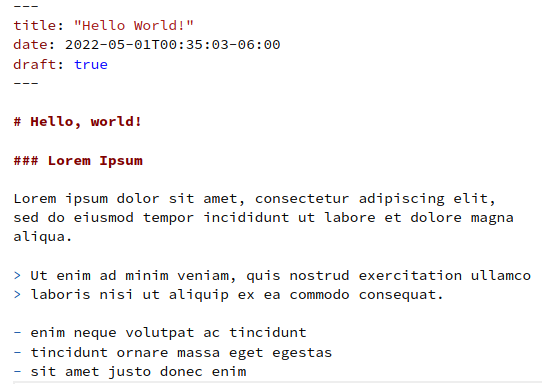
\includegraphics[width=\textwidth]{images/markdown.png}
        \end{column}
        \pause
        \begin{column}[c]{.1\textwidth}
            $$ \to $$
        \end{column}
        \begin{column}[T]{.45\textwidth}
            ...and turns it into a webpage:\ \\
            \smallskip
            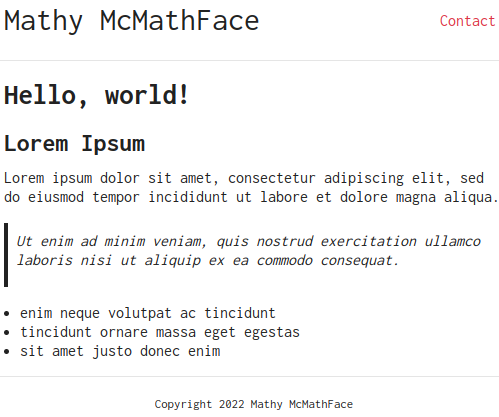
\includegraphics[width=\textwidth]{images/rendered_markdown.png}
        \end{column}
    \end{columns}

    \pause
    \vfill

    In many ways, Hugo does for webpages what \LaTeX \: does for documents.
    
\end{frame}
\begin{frame}
    \frametitle{Getting Started}

    First, we need to open a command line. The command line (also known as a terminal or console) is
    an invaluable tool for executing text commands on a computer.
    \medskip
    
    \begin{columns}
        \begin{column}{.45\textwidth}
            \begin{block}{Windows}
                From the Start Menu, open the \texttt{Git Bash} application:
                
\includegraphics[width=\textwidth]{images/windows_gitbash.png}
            \end{block}
        \end{column}

        \begin{column}{.45\textwidth}
            \begin{block}{MacOS}
                Open the \texttt{Terminal} application from Launchpad:
                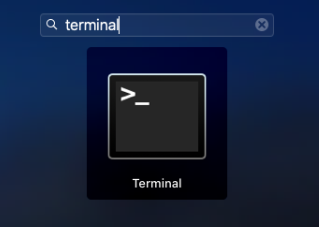
\includegraphics[width=\textwidth]{images/macos_terminal.png}
            \end{block}
        \end{column}
    \end{columns}
\end{frame}
\begin{frame}[fragile]
    \frametitle{Getting Started}

    Now we'll change directories (\texttt{cd}) to the \texttt{Desktop} folder.  Type the following into your terminal
    (\textbf{without} the "\$" character\footnote{
        It is customary to add this character in technical documentation to indicate that the proceeding
        command is to be entered into a terminal.
    }), and then hit the \texttt{[Enter]} key:
   
    \bigskip
    
    \begin{lstlisting}[style=saneCode,gobble=8]
        $ cd Desktop
    \end{lstlisting}

    \vfill
    Next, we'll use Git to clone (download) all the necessary code for this project. Type the following command into
    your terminal, and then hit the \texttt{[Enter]} key:

    \bigskip

    \begin{lstlisting}[style=saneCode,gobble=8]
        $ git clone https://github.com/uccs-ams/website-workshop.git --recurse
    \end{lstlisting}


\end{frame}
\begin{frame}[fragile]
    \frametitle{Getting Started}

    Let's change directories again to the newly-created \texttt{website-workshop} folder:
   
    \bigskip
    
    \begin{lstlisting}[style=saneCode,gobble=8]
        $ cd website-workshop
    \end{lstlisting}

    \vfill

    The next command we need to run depends on our operating system. We're going to check out slightly different
    versions of the code to account for operating system differences:

    \medskip

    \begin{block}{Windows}
    \begin{lstlisting}[style=saneCode,gobble=8]
        $ git checkout windows
    \end{lstlisting}
    \end{block}
    
    \begin{block}{MacOS}
    \begin{lstlisting}[style=saneCode,gobble=8]
        $ git checkout macos
    \end{lstlisting}
    \end{block}

    \begin{block}{MacOS [M1]}
    \begin{lstlisting}[style=saneCode,gobble=8]
        $ git checkout macos-arm64
    \end{lstlisting}
    \end{block}

\end{frame}
\begin{frame}[fragile]
    \frametitle{Start Hugo}

    We're finally ready to build our website! We first need to start our Hugo server, which lets us see our website
    in a browser and rebuilds the site automatically whenever we modify any project files:

    \bigskip

    \begin{lstlisting}[style=saneCode,gobble=8]
        $ ./hugo -D serve
    \end{lstlisting}

    \bigskip

    After running this command, we can see our website by navigating to \url{http://localhost:1313/} in a web
    browser. It'll be blank for now, but we're about to fix that.
\end{frame}
\begin{frame}[fragile]
    \frametitle{Website Scaffolding}

    Basic information about our website (title, theme, website URL, etc.) is contained in the \texttt{config.toml} 
    configuration file inside the \texttt{website-workshop} folder on our Desktop. 
    
    \medskip

    Let's open that file with a text editor and replace the existing content with the following to enable the
    \texttt{researcher} Hugo theme:

    \bigskip

    \begin{lstlisting}[style=saneCode,gobble=8,title={config.toml},numbers=left]
        baseURL = "http://example.org/" # If you have your own domain name, add it here.
        title = "Mathy McMathFace"
        theme = "researcher"
    \end{lstlisting}

    \vfill

    We're going to add quite a few more things to this file before we're done.
\end{frame}
\begin{frame}[fragile]
    \frametitle{Website Scaffolding}

    Now we'll update some basic page properties. This includes a navigation link to our resume and a page footer.

    \bigskip
    
    Be sure to pay attention to spacing!

    \medskip

    \begin{lstlisting}[style=saneCode,gobble=8,title={config.toml [ctd.]},numbers=left,firstnumber=4]
        [params]
          [params.footer]
            text = 'By Mathy McMathFace'
        
        [menu]
          [[menu.main]]
            name = "Resume"
            url = "/resume.pdf"
            weight = 1
    \end{lstlisting}

    \vfill

    Let's see what our website looks like so far.
\end{frame}
\begin{frame}[fragile]
    \frametitle{Main Page}

    Our \textbf{index} (main) page is looking pretty barren - let's change that! Our first task is to create a new 
    Markdown file for Hugo to turn into a webpage, and we'll use Hugo to do so.    

    \smallskip

    Open a new terminal, and then run the following command to navigate to our project directory:

    \medskip

    \begin{lstlisting}[style=saneCode,gobble=8]
        $ cd Desktop/website-workshop
    \end{lstlisting}

    \vfill

    From here, we'll instruct Hugo to generate a new Markdown file for us to modify:\footnote{
      The \texttt{\_index.md} file name holds special significance in Hugo projects; the contents of this file are
      rendered to the main page.
    }

    \medskip

    \begin{lstlisting}[style=saneCode,gobble=8]
        $ ./hugo new _index.md
    \end{lstlisting}

    \smallskip

    This command generates a new Markdown file at \texttt{website-workshop/content/\_index.md}.
\end{frame}
\begin{frame}[fragile]
    \frametitle{Main Page}
    
    This is our first encounter with actual Markdown code. Let's open our newly-generated file
    in a text editor and add some information in order to introduce ourselves to the world:

    \vfill

    \begin{lstlisting}[style=saneCode,gobble=8,title={content/\_index.md},numbers=left]
        ---
        title: "Mathy McMathFace"
        date: 2022-05-01T17:53:23-06:00  # This is auto-generated - no need to modify this!
        #draft: true
        ---
        
        # About
        
        ## PhD Student - University of Colorado at Colorado Springs
        
        &nbsp;
        **Mathy McMathface** is currently a graduate student studying Mathematics
        at the University of Colorado at Colorado Springs (UCCS) and is an officer for
        the American Mathematical Society Graduate Student Chapter at UCCS. Their
        research interests include inverse reactive currents for use in unilateral
        phase detractors, automatic cardinal grammeter synchronization, and how these
        two may be combined in various ways to create turbo encabulators.
    \end{lstlisting}
\end{frame}
\begin{frame}[fragile]
    \frametitle{Contact Page}

    Now that the world knows who we are, let's create a contact page so that they know how to reach us.
    Like before, we'll use Hugo to generate a new page:

    \medskip

    \begin{lstlisting}[style=saneCode,gobble=6]
      ./hugo new contact.md
    \end{lstlisting}

    \vfill

    We also need to add a link to this page from our index page. We can add links to pages by modifying our 
    \texttt{config.toml} configuration file, just like we did before for our resume:

    \begin{lstlisting}[style=saneCode,gobble=6,title={config.toml},numbers=left,firstnumber=8]
      ...
      [menu]
        [[menu.main]]
          name = "Resume"
          url = "/resume.pdf"
          weight = 1
        [[menu.main]]
          name = "Contact"
          url = "/contact"
          weight = 2
    \end{lstlisting}
\end{frame}
\begin{frame}[fragile]
    \frametitle{Contact Page}

    This page gives us the opportunity to see some new Markdown syntax for quote blocks and hyperlinks:
    
    \begin{lstlisting}[style=saneCode,gobble=8,title={content/contact.md},numbers=left]
        ---
        title: "Contact"
        date: 2022-05-01T18:22:37-06:00
        #draft: true
        ---
        
        # Contact
                
        &nbsp;
        ## E-mail
        Feel free to e-mail me at [mmcmath@uccs.edu](mailto:mmcmath@uccs.edu).
        
        &nbsp;
        ## Mailing Address
        > University of Colorado at Colorado Springs
        > 
        > Department of Mathematics 
        > 
        > 1420 Austin Bluffs Parkway
        > 
        > Colorado Springs, CO 80918 
    \end{lstlisting}
\end{frame}
\begin{frame}[fragile]
    \frametitle{Posts Page}

    We can also use Hugo to easily create and manage blog posts:

    \medskip

    \begin{lstlisting}[style=saneCode,gobble=8]
        $ ./hugo new posts/hello-world.md
    \end{lstlisting}

    \vfill
    As before, we'll add a link to our new \texttt{Posts} page:

    \begin{lstlisting}[style=saneCode,gobble=6,title={config.toml},numbers=left,firstnumber=8]
      ...
      [menu]
        [[menu.main]]
          name = "Resume"
          url = "/resume.pdf"
          weight = 1
        [[menu.main]]
          name = "Contact"
          url = "/contact"
          weight = 2
        [[menu.main]]
          name = "Posts"
          url = "/posts"
          weight = 3
    \end{lstlisting}
\end{frame}
\begin{frame}[fragile]
    \frametitle{Posts Page}

    We've seen up to this point that Markdown provides some pretty basic formatting out of the box.
    What if we want \LaTeX \: in our blog posts?

    \vfill

    \begin{lstlisting}[style=saneCode,gobble=8,title={content/posts/hello-world.md},numbers=left]
        ---
        title: "Hello World"
        date: 2022-05-01T15:58:31-06:00
        #draft: true
        math: true
        ---

        # Hello, world!

        This is my first blog post. In this post, I will do things like:

        - Make lists
        - _Emphasize_ text
        - Make text **bold**
        - Show off some inline $\LaTeX$
    \end{lstlisting}
\end{frame}
\begin{frame}[fragile]
    \frametitle{Back to the Beginning}

    At this point, we have created a basic website with Hugo by creating several Markdown pages. We now need to convert
    these files into HTML, CSS, and JavaScript so that our website can be hosted on the public internet.

    \bigskip

    To do so, we simply run the following from our terminal:

    \smallskip

    \begin{lstlisting}[style=saneCode,gobble=8]
        $ ./hugo
    \end{lstlisting}

    \bigskip
    Our compiled websites files can then be found in the \texttt{public} folder in our project directory.
\end{frame}
\begin{frame}[c]

    \begin{center}
        \Huge Questions?
    \end{center}

\end{frame}

% Appendices
\begin{frame}[fragile]
    \frametitle{Appendix: Hosting}

    Now that we've built a basic website, we need somewhere to host it so that it is accessible on the public internet.
    There are two steps to this process:

    \smallskip

    \begin{enumerate}
        \item Choosing a domain name (e.g., example.org)
        \item Choosing a hosting service
    \end{enumerate}

    \medskip
    Choosing a hosting service is outside the scope of this workshop, but some good places to start are:

    \smallskip

    \begin{itemize}
        \item \href{https://www.bluehost.com/}{Bluehost}
        \item \href{https://www.namecheap.com}{Namecheap}
        \item \href{https://www.hostgator.com/}{HostGator}
    \end{itemize}

    \vfill

    Each of these services provide both domain registration and website hosting services.
\end{frame}
\begin{frame}[fragile]
    \frametitle{Appendix: Hugo Themes}

    Hugo's support for various site themes makes it easy to change the look and feel of our website.
    In this workshop, we used the excellent \href{https://themes.gohugo.io/themes/hugo-researcher/}{Researcher} theme
    for its academic look and feel, but a full list of themes can be found at \url{https://themes.gohugo.io/}.

    \vfill

    To change a theme (e.g., to the \href{https://themes.gohugo.io/themes/gohugo-theme-ananke/}{Ananke theme}), we
    first clone (download) the theme to our project by running the following from our terminal (as before, the entire 
    command should be on a single line):

    \vfill

    \begin{lstlisting}[style=saneCode,gobble=8]
        $ git submodule add https://github.com/theNewDynamic/gohugo-theme-ananke.git themes/ananke
    \end{lstlisting}
\end{frame}
\begin{frame}[fragile]
    \frametitle{Appendix: Hugo Themes}

    Next, we update the active theme in our project's \texttt{config.toml} configuration file:

    \medskip

    \begin{lstlisting}[style=saneCode,gobble=8,title={config.toml},numbers=left]
        baseURL = "http://example.org/" # If you have your own domain name, add it here.
        title = "Mathy McMathFace"
        theme = "ananke"
        ...
    \end{lstlisting}

    \vfill

    In general, configuration options for a particular theme (e.g., to change background or text color) can usually 
    be found in the corresponding example configuration file for that theme at
    \texttt{themes/<theme name>/exampleSite/config.toml}.

\end{frame}

\end{document}